\subsection{Specyfikacja wymagań na produkt programowy}

\begin{figure}[!htb]
    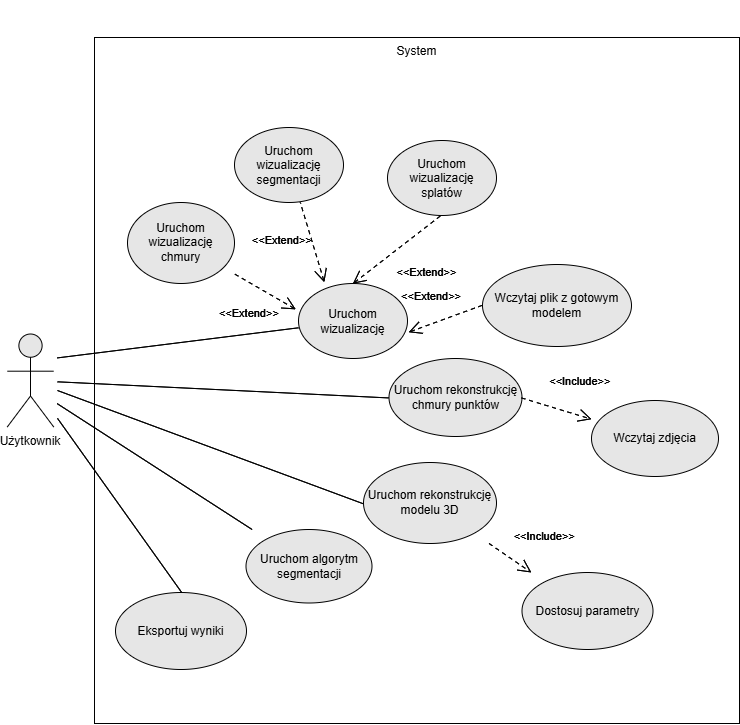
\includegraphics[width=1.0\linewidth]{img/diagramy/zpi use case.png}
    \caption{Diagram przypadków użycia}\label{fig:use_case_diagram}
  \end{figure}

\clearpage

\subsection{Architektura}

\begin{figure}[!htb]
    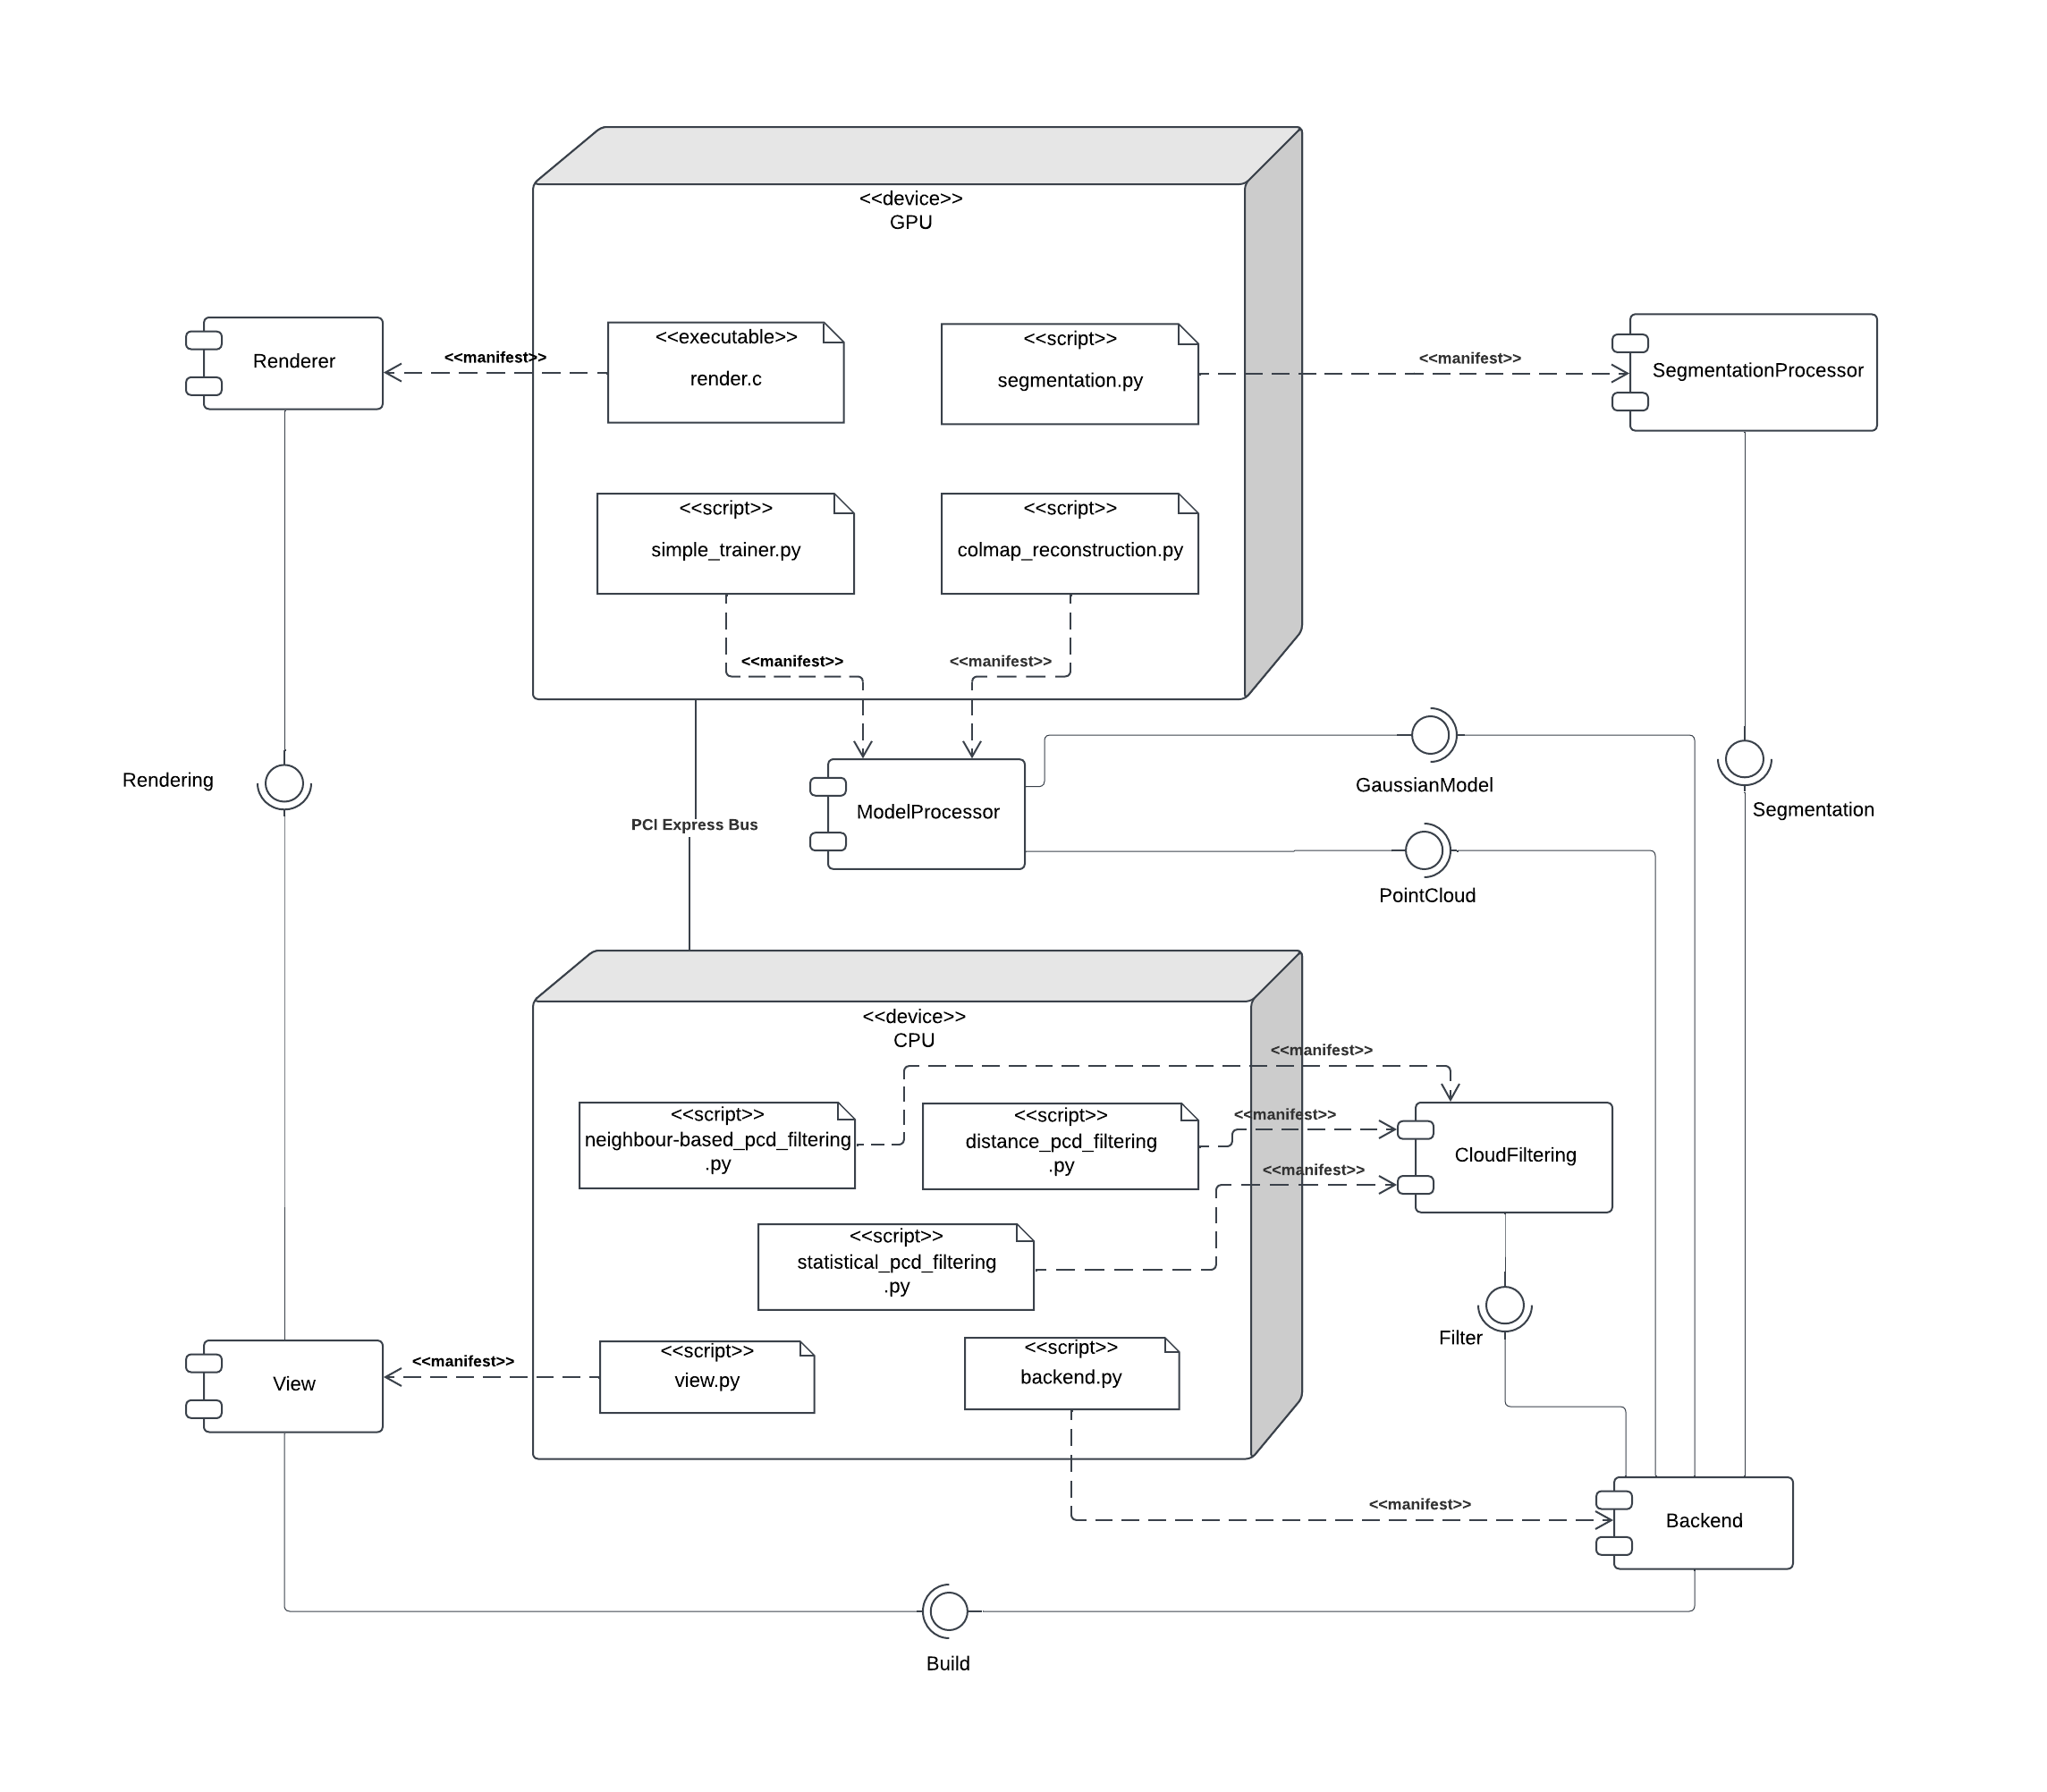
\includegraphics[width=1.0\linewidth]{img/diagramy/diagram_wdrozenia_komponentow_3.png}
    \caption{Diagram wdrożenia komponentów}\label{fig:components_diagram}
\end{figure}

\subsubsection{Architektura}
Projekt został zrealizowany w oparciu o wzorzec projektowy \textbf{MVVM} (Model-View-ViewModel), który został odpowiednio dostosowany do specyfiki aplikacji w celu zapewnienia modularności oraz uproszczenia procesu modyfikacji i rozbudowy.

\textbf{Adaptacja wzorca MVVM}
\begin{figure}[h!]
    \centering
    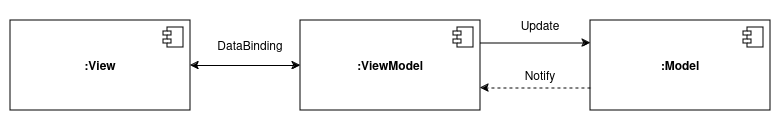
\includegraphics[width=0.8\textwidth]{img/diagramy/architektura.png}
    \caption{Schemat zaadaptowanego wzorca MVVM w projekcie.}
\end{figure}

W zaimplementowanym rozwiązaniu wzorzec \textbf{MVVM} został zmodyfikowany w celu optymalizacji komunikacji między komponentami aplikacji. Dzięki temu możliwe było osiągnięcie spójności architektury oraz jej wysokiej skalowalności.

\paragraph{Opis komponentów architektury}
\begin{figure}[h!]
    \centering
    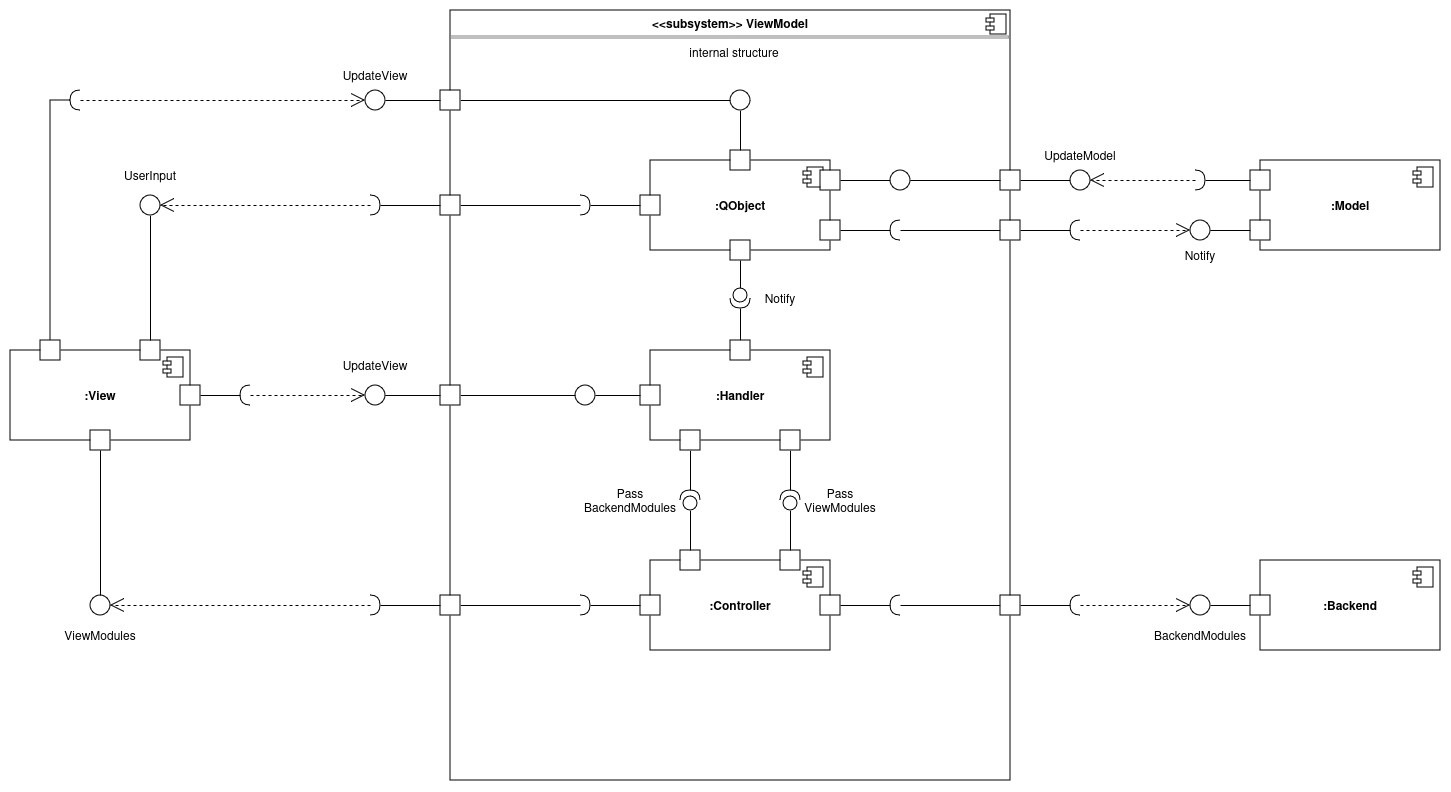
\includegraphics[width=0.8\textwidth]{img/diagramy/diagram_komp_vm.png}
    \caption{Struktura komponentów ViewModel w projekcie.}
\end{figure}

W projekcie klasa \texttt{ViewModel} zastępuje tradycyjny zbiór klas, takich jak:
\begin{itemize}
    \item \texttt{Controller} -- odpowiadający za sterowanie logiką,
    \item \texttt{QObject} -- obsługujący komunikację z frontendem,
    \item \texttt{Handler} -- integrujący dodatkowe funkcjonalności wizualne.
\end{itemize}

\textbf{Rola \texttt{QObject}}
Klasa \texttt{QObject} pełni funkcję tradycyjnego komponentu \texttt{ViewModel}, umożliwiając komunikację między warstwą logiki a frontendem aplikacji. Wykorzystuje mechanizm sygnałów dostarczany przez bibliotekę PyQt, co pozwala dynamicznie informować widok o zmianach stanu aplikacji.

\textbf{Handler jako rozszerzenie funkcjonalności}
\texttt{QObject} został wzbogacony o klasę \texttt{Handler}, która pozwala na łatwą implementację funkcji wizualnych w już istniejącej architekturze. Dzięki temu projekt zachowuje przejrzystość i elastyczność.

\textbf{Integracja za pomocą \texttt{Controller}}
Klasy \texttt{QObject} i \texttt{Handler} są zintegrowane za pomocą \texttt{Controller}, który zapewnia jednolity interfejs oraz ułatwia zarządzanie komponentami aplikacji.

Na diagramie widoczny jest dodatkowy komponent \textbf{Backend}, będący zbiorem skryptów, które dostarczają interfejs dla wymaganej funkcjonalności aplikacji. Backend odpowiada za obsługę logiki niezwiązanej bezpośrednio z widokiem oraz wspiera pozostałe komponenty architektury, zapewniając większą modularność.

\paragraph{Zalety wdrożonego rozwiązania}
Przedstawione rozwiązanie zapewnia następujące korzyści:
\begin{itemize}
    \item \textbf{Modularność} -- możliwość łatwego dodawania i modyfikowania komponentów bez ingerencji w istniejącą strukturę.
    \item \textbf{Skalowalność} -- umożliwia rozbudowę aplikacji o nowe funkcjonalności przy zachowaniu spójności architektury.
    \item \textbf{Wsparcie dla współbieżności} -- dzięki zastosowaniu mechanizmu sygnałów PyQt implementacja współbieżności jest intuicyjna i efektywna.
\end{itemize}

\paragraph{Podsumowanie}
Zaimplementowany wzorzec MVVM, w połączeniu z dodatkowymi modyfikacjami, pozwolił osiągnąć elastyczną i skalowalną architekturę aplikacji. Dzięki zastosowanemu podejściu projekt spełnia założenia modularności, umożliwiając łatwą rozbudowę oraz utrzymanie w przyszłości.

% \subsection{Implementacja}

\subsection{Wizualizacja}
W celu zapewnienia użytkownikowi końcowemu zintegrowanego i spójnego środowiska wizualizacji całego procesu – od wgrania plików wejściowych po interakcję z modelem – zaprojektowano od podstaw interfejs oraz system renderowania.

Założeniem projektu była implementacja intuicyjnego, dynamicznego i responsywnego \textbf{interfejsu}[\ref{fig:ui}] przy pomocy biblioteki \textit{PyQt} oraz języka \textit{QML}. Interfejs został zintegrowany z wydajnym systemem \textbf{renderingu}[\ref{fig:rendering}] GPU, wykorzystującym technologie \textit{OpenGL}, \textit{OpenCL} oraz język \textit{C}. Dodatkowo, użytkownik ma możliwość alternatywnego renderowania z wykorzystaniem biblioteki \textit{VisPy}.

Projekt rozwiązuje problem fragmentaryczności funkcji dostępnych w innych aplikacjach, oferując spójne środowisko do obsługi modeli 3D, obejmujące procesy tworzenia, modyfikacji, segmentacji oraz wizualizacji danych.
\\[10pt]
\textbf{Funkcjonalności interfejsu}

\begin{itemize} \item wybór zdjęć, \item ustawienie parametrów, \item generowanie chmury punktów, \item generowanie splatów, \item segmentacja splatów, \item wizualizacja wyników. \end{itemize}

\vspace{10pt}
{\setlength{\parindent}{0pt}
\textbf{Rendering}
}

Rendering wykorzystuje plik .ply jako dane wejściowe do wczytania splatów. Splaty te są reprezentowane przez sześciany z dodatkowymi parametrami przechowywanymi w Shader Storage Buffer Object (SSBO), co umożliwia efektywny odczyt dużych ilości danych. Takie podejście jest szczególnie przydatne w przypadku scen zawierających nawet do dwóch milionów obiektów.

Do przechowywanych parametrów należą: \begin{itemize} \item pozycja, \item skala, \item rotacja, \item kolor, \item przezroczystość. \end{itemize}

Podczas procesu renderowania, model sześcianu jest odpowiednio przekształcany na podstawie tych parametrów, co pozwala na uzyskanie splatów na wyjściu. Takie podejście umożliwia abstrakcyjne definiowanie splatów przy jednoczesnym zachowaniu wysokiej dokładności wizualnej.

\clearpage

\begin{figure}[!ht]
    \centering
    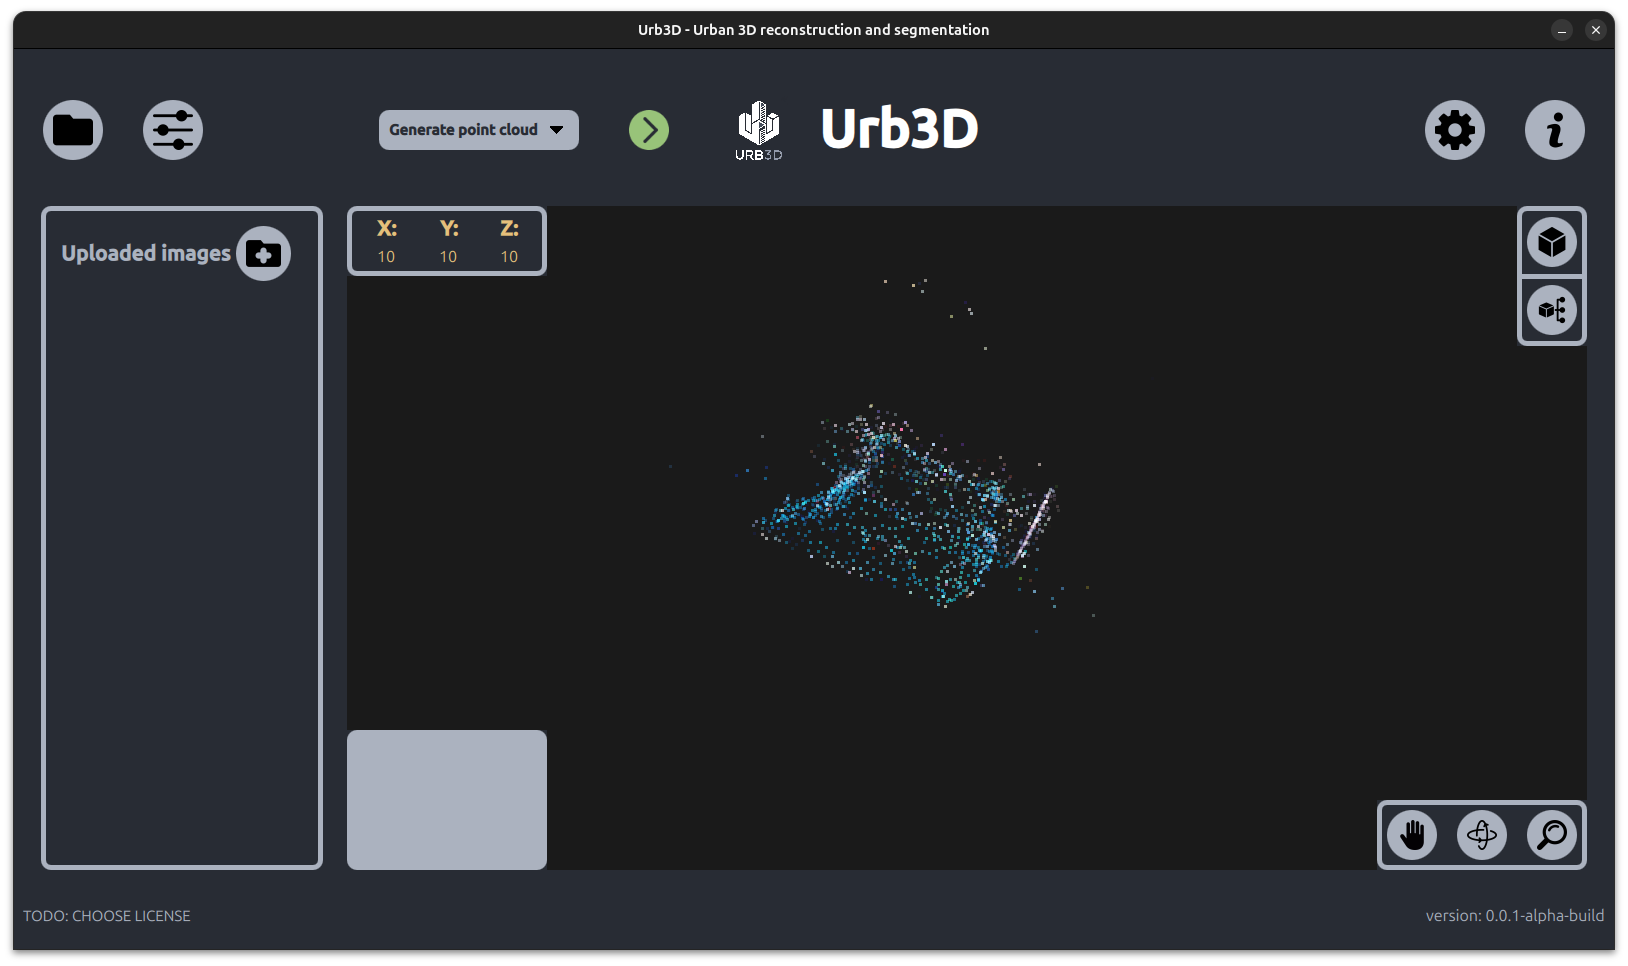
\includegraphics[width=\textwidth]{images/UI-Rendering.png}
    \caption{Zrzut ekranu przedstawiający główny widok aplikacji}
    \label{fig:ui}
\end{figure}

\begin{figure}[!ht]
    \centering
    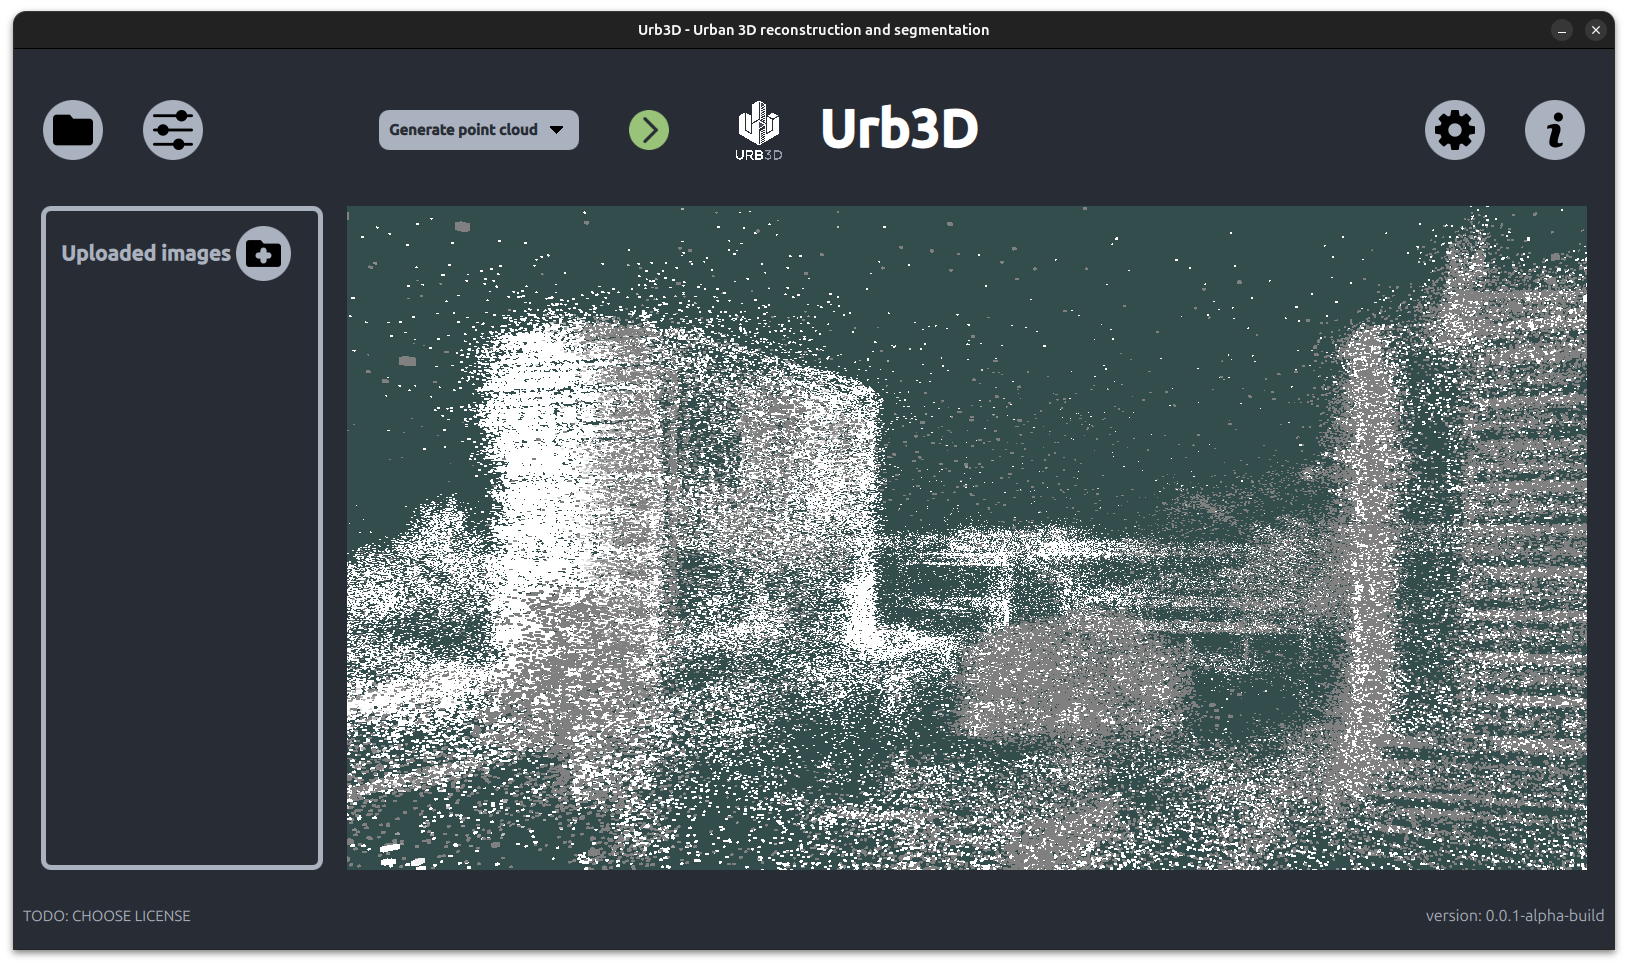
\includegraphics[width=\textwidth]{images/cloud_rendering.png}
    \caption{Zrzut ekranu przedstawiający własny renderer}
    \label{fig:rendering}
\end{figure}

\subsection{Rendering}

W aplikacji zaimplementowano autorski system renderingu w celu zapewnienia wysokiej wydajności oraz wygody użytkowania przez użytkownika końcowego. Do realizacji tego rozwiązania wykorzystano język C oraz bibliotekę OpenGL z rozszerzeniami GLEW, GLFW i CGLM.

\begin{figure}[h!]
    \centering
    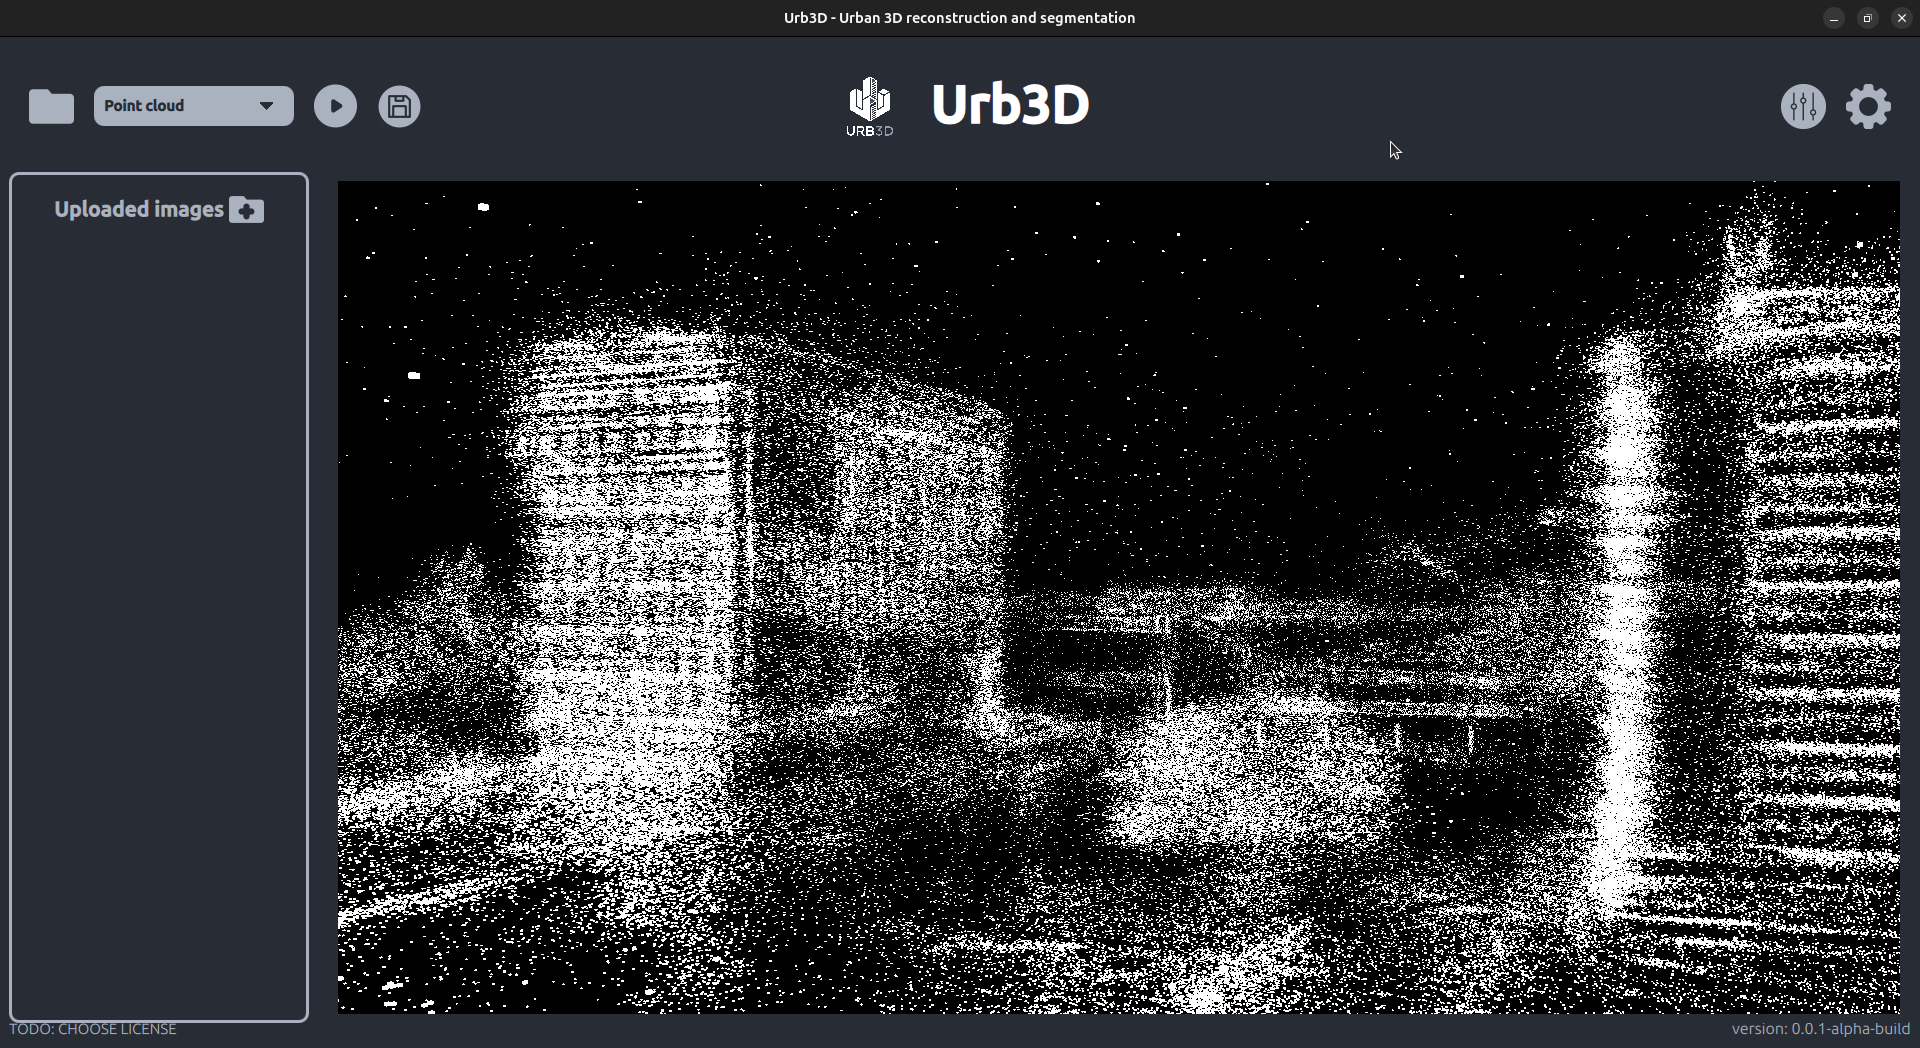
\includegraphics[width=0.8\textwidth]{img/wizualizacja/ui_rendering.png}
    \caption{Widok główny aplikacji z zaimplementowanym renderingiem.}
    \label{fig:widok_glowny}
\end{figure}

\subsubsection{Integracja z Pythonem}
Rendering został udostępniony jako dynamiczna biblioteka współdzielona, co umożliwia jego integrację z aplikacjami napisanymi w języku Python. Dzięki temu, w połączeniu z frameworkiem PyQt, rendering może być efektywnie wykorzystywany w aplikacjach graficznych.

\begin{figure}[h!]
    \centering
    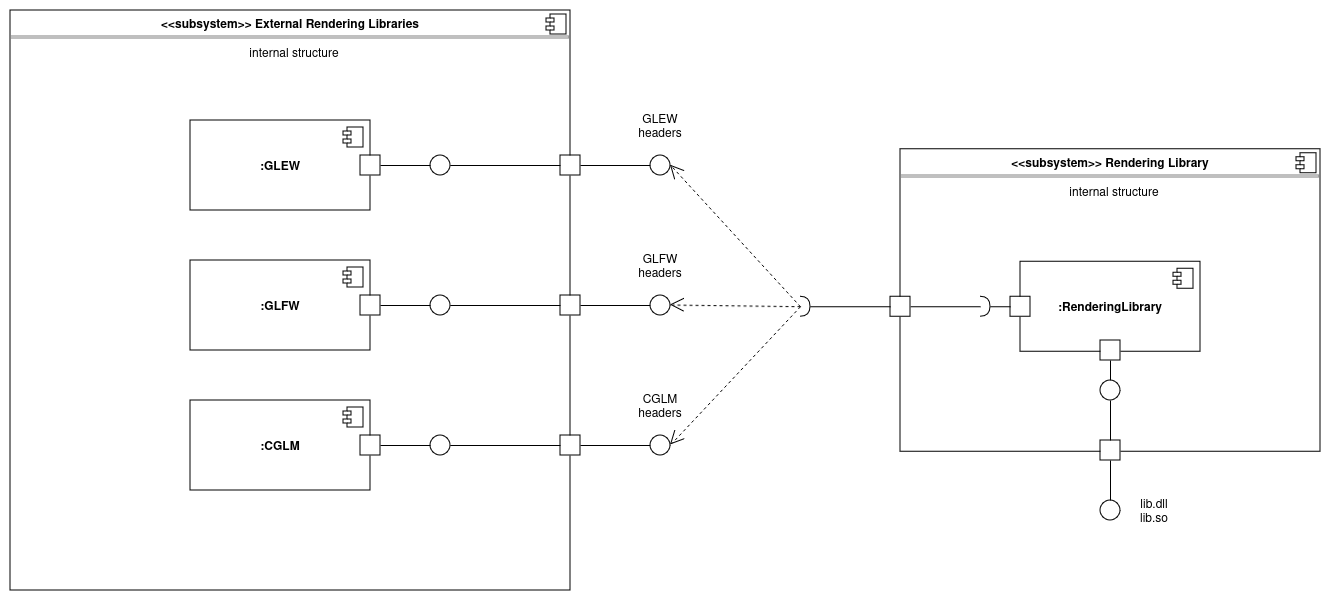
\includegraphics[width=0.8\textwidth]{img/diagramy/diagram_komp_rendering.png}
    \caption{Diagram przedstawiający architekturę integracji renderingu z Pythonem.}
    \label{fig:diagram}
\end{figure}

\subsubsection{Implementacja systemu renderingu}

\textbf{Reprezentacja punktów i splatów}
Wizualizacja punktów oraz splatów została zrealizowana za pomocą sześcianów, które są skalowane i rotowane w taki sposób, aby przypominały elipsoidy. Przetworzone w ten sposób sześciany są następnie renderowane przy użyciu shaderów, co pozwala na uzyskanie efektu ich zaokrąglenia.

\textbf{Optymalizacja wydajności}
Aby zwiększyć wydajność obliczeń graficznych, wykorzystano GPU z użyciem obiektów SSBO (Shader Storage Buffer Objects). SSBO umożliwiają przechowywanie i przetwarzanie dużych ilości danych bezpośrednio na karcie graficznej, co minimalizuje obciążenie procesora głównego.

\clearpage

W ramach procesu renderingu wczytywane są dane statyczne dla domyślnego sześcianu, a następnie przetwarzane są atrybuty poszczególnych punktów, takie jak:
\begin{itemize}
    \item pozycja,
    \item skalowanie,
    \item rotacja,
    \item przezroczystość,
    \item kolor.
\end{itemize}

Takie podejście zapewnia elastyczność oraz wysoką wydajność w generowaniu scen 3D.

% \clearpage

\subsection{Technologie}

W projekcie wykorzystano następujące technologie

\begin{itemize}
    \item \textbf{C/C++}: OpenCL, OpenGL
    \item \textbf{Python}: Pytorch, pycolmap, open3d, pyvista, PyQt (numpy, matplotlib), pytest
    \item CloudCompare, Meshlab
    \item \textbf{GPU}
    \item Jira, Confluence, Github, Discord
\end{itemize}

\begin{figure}[!ht]
    \centering
    
\includegraphics[width=0.9\linewidth]{img/sota/technologie.png}
  \end{figure}

\subsubsection{Struktura plikowa projektu}

% millon opcji https://tex.stackexchange.com/questions/5073/making-a-simple-directory-tree
\begin{forest}
  for tree={
    grow'=0,
    child anchor=west,
    parent anchor=south,
    anchor=west,
    calign=first,
    edge path={
      \noexpand\path [draw, \forestoption{edge}] (!u.south west) ++(3pt,0) -- +(-3pt,0) |- (.child anchor)\forestoption{edge label};
    },
    before typesetting nodes={
      if n=1
        {insert before={[,phantom]}}
        {}
    },
    fit=band,
    before computing xy={l=15pt},
  }
[project
  [data
    [city\_model
      [images]
      [sparse
          [images.bin]
          [cameras.bin]
          [points.bin]
          [sparse.ply]
      ]
      [filtered\_model.ply]
      [model.pt]
      [model.ply]
      [model\_seg.ply]
    ]
    [pointnet-ckpt.pt]
  ]
  [scripts]
  [src
    [frontend]
    [backend]
    [urb3d
      [datasets]
      [pipeline]
      [segmentation]
      [rendering]
      [geometry]
      [models]
      [splats]
    ]
  ]
  [test]
]
\end{forest}